\section{Overview}

In this chapter, we present a framework called \ToolP that provides a view-centric 
and database-aware analysis
for web developers to understand and optimize 
their database-backed web applications. \ToolP currently targets applications  written using the Ruby on Rails framework, and makes three major contributions as illustrated in Figure \ref{fig:overview}.

\ToolP provides a view-centric estimator that helps developers understand the 
data-processing cost behind every HTML tag. 
\ToolP both dynamically monitors database query performance using the test workload, statically estimates data processing complexity independent of any specific workload, and carefully attributes the cost to every HTML tag
through its cross-stack dependency analysis. The details will be presented in 
Section \ref{sec:profile}.

\ToolP provides a view-aware performance optimizer that helps developers carry out
view-changing code refactoring to improve performance. \ToolP suggests a variety
of refactorings that (1) change the manner of content rendering (i.e., pagination or asynchronous loading);
or (2) change the accuracy of the rendered contents (i.e., approximation);
or (3) remove certain web-page contents from rendered contents. Through static program
analysis, \ToolP not only identifies opportunities for applying such refactoring,
but also automatically suggests patches that complete such refactoring,
often involving modifications to multiple files in model, view, and controller components.
We present the details in Section \ref{sec:opt}.

%We estimates the performance cost for each HTML tag that will be rendered on the page through dynamic run-time logging and static analysis, which is a new granularity for performance estimation. Also our approach includes the wall-clock performance cost and relative performance cost towards the database size. As a result, this approach also works when there is not a representative workload for us to gain enough performance cost information. 

\ToolP provides a unique interface for developers to effectively
exploring different web-page designs with different performance-functionality trade-offs.
Instead of separately presenting profiling information and refactoring suggestions, \ToolP integrates them in the web browser---while testing a page of their web applications, the data processing cost for each HTML tag is presented as a heat map in the browser. Developers can right click on each
HTML tag to see the different view-changing options for performance enhancement; they can 
choose any option and immediately see an updated web page with an updated heat map in the browser,
with all code refactoring automatically done by \ToolP in an accompanying Ruby editor.
%Section \ref{sec:im} explains how \ToolP implements this interface through a combination of
%Ruby editor plug-ins, \ToolP performance-debugging JavaScript, and static instrumentation 
%of the web application under development.

%Users can easily explore various types of optimizations 
%before they decide on the most suitable design that gives the 
%best balance between web-page functionality and page-loading performance. 
%\alvin{this paragraph seems to be more of a description of how \ToolP works. I suggest moving this somewhere else and state precisely what is new about the \ToolP interface here instead}

%Secondly, we implement this approach into a prototype on Ruby on Rails framework through Rails libraries and RubyMine IDE plugin. 




\begin{figure}
    \centering
    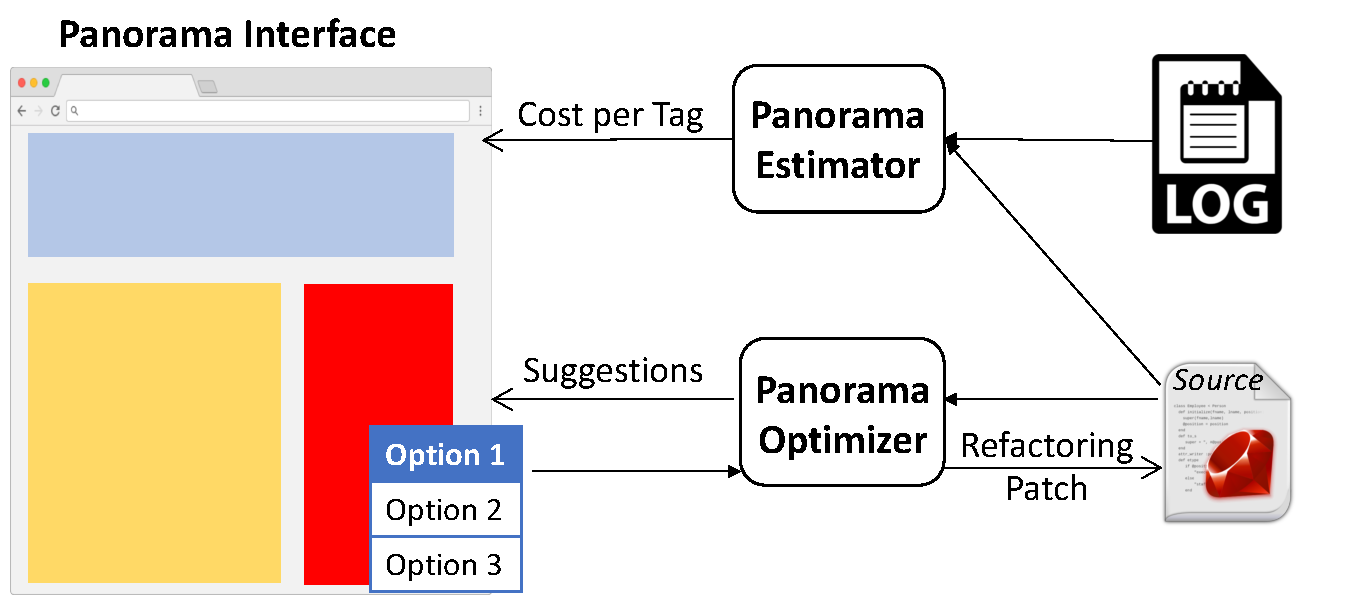
\includegraphics[width=0.7\columnwidth]{panorama-figs/overview.pdf}
    \vspace{-0.1in}
    \caption{\ToolP overview}
     \vspace{-0.2in}
    \label{fig:overview}
\end{figure}


We evaluated \ToolP on 12 popular open-source Ruby on Rails applications.
\ToolP statically identifies \numissues performance-enhancing
opportunities through view changes. We randomly sampled 15 view changes suggested
by \ToolP and found that by applying the patches automatically generated by \Tool,
these 15 view changes speed up end-to-end page load time by \eoespeedup on average
(\maxspeedup maximum), using database workloads that are similar to those used in real-world deployments. We believe the benefits will increase with even larger workloads. %a larger workload will offer even bigger speedup.
Furthermore, we conducted a thorough user study with 100 participants from
Amazon Mechanical Turk. The study shows that web pages with these
view changes are considered as similar or better than the original web pages
in most cases, with more users preferring the design suggested by
\ToolP than the original ones. This user study result, as well as the fact 
that these optimizations save computation resources on web servers and database servers, justify the need for developers to explore the performance-functionality 
trade-off space in web application design, with \ToolP being a first step towards that goal.